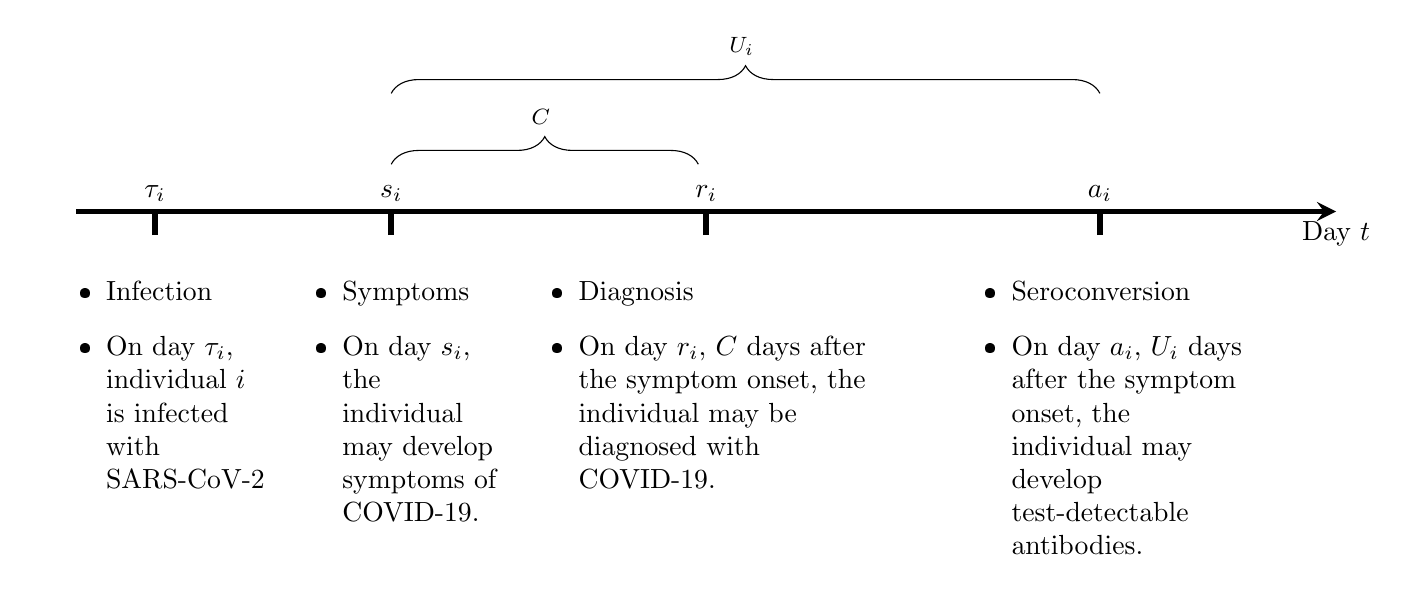
\begin{tikzpicture}
\usetikzlibrary{calc}

% draw arrow
\coordinate (start) at (-1,0);
\coordinate (end) at (15,0);
\draw [line width=2pt, -stealth] (start) -- (end);

% You can use `foreach` to improve the following codes
\coordinate (s0) at (0,-0.3);
\coordinate (t0) at ($(s0)+(0,0.3)$);
\coordinate (s1) at (3,-0.3);
\coordinate (t1) at ($(s1)+(0,0.3)$);
\coordinate (s2) at (7,-0.3);
\coordinate (t2) at ($(s2)+(0,0.3)$);
\coordinate (s3) at (12,-0.3);
\coordinate (t3) at ($(s3)+(0,0.3)$);

\node [anchor=north] at (end.south) {\text{Day} $t$};

% draw ticks
\draw [line width=2pt] (s0) -- (t0);
\node [anchor=south] at (t0.north) {$\tau_i$};

\draw [line width=2pt] (s1) -- (t1);
\node [anchor=south] at (t1.north) {$s_i$};

\draw [line width=2pt] (s2) -- (t2);
\node [anchor=south] at (t2.north) {$r_i$};

\draw [line width=2pt] (s3) -- (t3);
\node [anchor=south] at (t3.north) {$a_i$};

% draw decorations

\draw [decorate,decoration={brace,amplitude=10pt},xshift=-3pt,yshift=0pt]
($(t1)+(0, 0.6)$) -- ($(t2)+(-0.1,0.6)$) node [black,midway,xshift=-0.05cm,yshift=0.6cm] 
{\footnotesize $C$};

\draw [decorate,decoration={brace,amplitude=10pt},xshift=-3pt,yshift=0pt]
($(t1)+(0, 1.5)$) -- ($(t3)+(0,1.5)$) node [black,midway,xshift=-0.05cm,yshift=0.6cm] 
{\footnotesize $U_i$};


% add texts
\node [anchor=north, align=left, text width=3cm] at (s0.south) {
\begin{itemize}
\item Infection 
\item On day $\tau_i$, individual $i$ is infected with SARS-CoV-2
\end{itemize}
};

\node [anchor=north, align=left, text width=3cm] at (s1.south) {
\begin{itemize}
\item Symptoms
\item On day $s_i$, the individual may develop symptoms of COVID-19.
\end{itemize}
};

\node [anchor=north, align=left, text width=5cm] at (s2.south) {
\begin{itemize}
\item Diagnosis
\item On day $r_i$, $C$ days after the symptom onset, the individual may be diagnosed with COVID-19.
\end{itemize}
};

\node [anchor=north, align=left, text width=4cm] at (s3.south) {
\begin{itemize}
\item Seroconversion
\item On day $a_i$, $U_i$ days after the symptom onset, the individual may develop test-detectable antibodies.
\end{itemize}
};

\end{tikzpicture}
